\documentclass[../thesis.tex]{subfiles}
\begin{document}
\chapter{Experimental Results of Standard Algorithms}
\label{ch:experimentsalgos}

The test suite runs all of the algorithms discussed above on a subset of stocks and generates profit figures for different denominations of stocks purchased. For every buy signal generated, the strategies ran on purchasing 10, 100, and 1000 stocks at a time. The strategies were implemented in Python and accessed stock data stored in csv files. The implementation leveraged Pandas Dataframes to store and manipulate the stock data. Pandas is a python data analysis package and is perhaps the most powerful open source data analysis or manipulation tool available. See Section 9.1 for pseudocode of each strategy's implementation.  The best way to understand how effective a particular strategy is to compare against a baseline, which is discussed above, helping us analyze the effectiveness of each strategy.   

\section{Momentum Strategies}

Standalone momentum strategies as a whole very rarely beat out the baseline measure. Figure 9 displays the results of AAPL, GOOG, HAS, QCOM, and AMD when using SMA, EMA, Bollinger Bands, and RSI. Only a few stocks had any strategies beat the baseline. One was GOOG, with both Bollinger Bands and RSI outperforming the baseline profit significantly. AMD for both SMA and EMA proved to be effective as well. However, for most it was more profitable to simply just buy and hold over the period. Figure~\ref{MOMENTUMfigure} demonstrates this poor performance. The baseline bar chart on the right side of the graph outperforms nearly every strategy. This however seems counterintuitive, as we should be generating profitable buying and selling trading signals with all of the computation, but that is clearly not the case.  Clearly, these strategies aren't viable as standalone trading algorithms. Now we will discuss why we observed overall poor performance.

The dual moving average algorithm when applied to both SMA and EMA isn't particularly effective. Due to the nature of SMA, which generally looks at long periods of time to highlight trends, this can induce a lagged effect to the buy and sell orders. A lagged effect in the context of moving averages is that the current moving average doesn't react to the current trend because of this longer observation window, often making this method ineffective. This lagged effect can be fixed by looking at an Exponential Moving Average analysis \cite{Ehlers}. However, unlike the literature suggests, in practice this doesn't translate to profit. AAPL nearly doubled its profit from using the exponential window that removes the lagged effect yet still had 2.53\% less returns than the baseline. While as a whole the strategy was more effective than SMA and did come closer to baseline performance, it rarely ended up beating it. This suggests that these indicators should be looked at in a different, combined context where multiple indicators could provide more robust trading signals. See the following section for discussion. 

With Bollinger Bands, buy and sell signals are still reliant on changes in rolling average prices. However, because of the incorporation of standard deviation, this strategy uses volatility in the market to further base buy and sell decisions. While a significant portion of the chosen stocks didn't end up actually out performing the baseline, a majority of them were within 1-2 percent performance of the baseline. 33\% of stocks tested on the strategy out performed each of its own baseline measure of buying and holding a specific denomination of shares throughout the entire period. Most notably, GOOG outperformed the baseline by 2.77\% while the implementations of SMA and EMA had abysmal performances of -30.25\% and -19.41\% respectively. While still not a passable standalone algorithm, the improvement over SMA and EMA is encouraging.

RSI takes advantage of over-purchasing or overselling of securities to predict convergence back to the mean. So, this strategy does take advantage of mean reversion. Unfortunately, most RSI implementations didn't outperform the baseline. The performance was comparable to EMA but slightly worse, as we see less stocks beating out the baseline. GOOG beat the baseline by 12.88\% while on the other hand DIS massively underperformed and posted a -7.08\% performance. 

\begin{figure}[h]
\centering
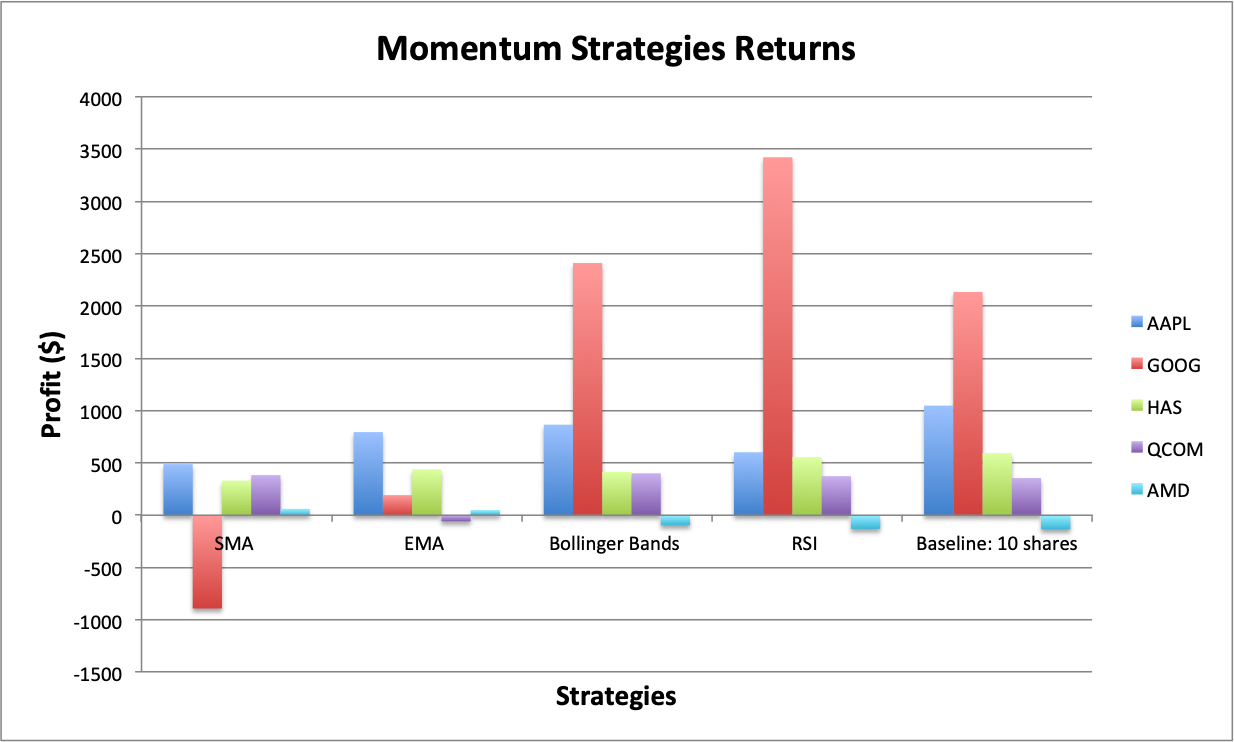
\includegraphics[width=.9\textwidth]{momentumstrategiesreturns.png}
\caption{Momentum Strategies Results  \label{overflow}}
\label{MOMENTUMfigure}
\end{figure}

\section{Combination Momentum Strategies}

The RSI and MACD combined implementation performed incredibly well. The most notable performances were from AAPL and HD. When purchasing 1000 shares at each buy signal, AAPL out-gained the baseline by \$9070  while HD had \$4990 of profit with the strategy while the baseline lost \$3750. Of all 30 stocks tested, only 3 stocks ended up with negative profit at the end of the day. AXP is a good example - generating a loss of \$1300 more than the baseline. With enough capital, this strategy could be used to generate incredible returns on a daily basis. Figure~\ref{RSIMACDRESULTSfigure} shows this strong performance. The green bar - the profit of the strategy buying or selling 1000 shares at a time, beats out the correspond baseline purple bar for every single stock, giving truly significant results. 

This algorithm generates incredibly robust buy signals and frequent sell signals which can nearly guarantee gains after buy signals. Therefore, utilizing strategies where 1000 shares of a given stock can generate massive profits with less risk of massive losses. It is also important that each transaction purchases a large amount of shares because it is necessary to offset the transaction cost charged by brokers. However, rather than focusing on individual stocks over time, this combination strategy is best implemented over a pool of multiple stocks because it isn't uncommon for days to generate absolutely no buy signals.

\begin{figure}[h]
\centering
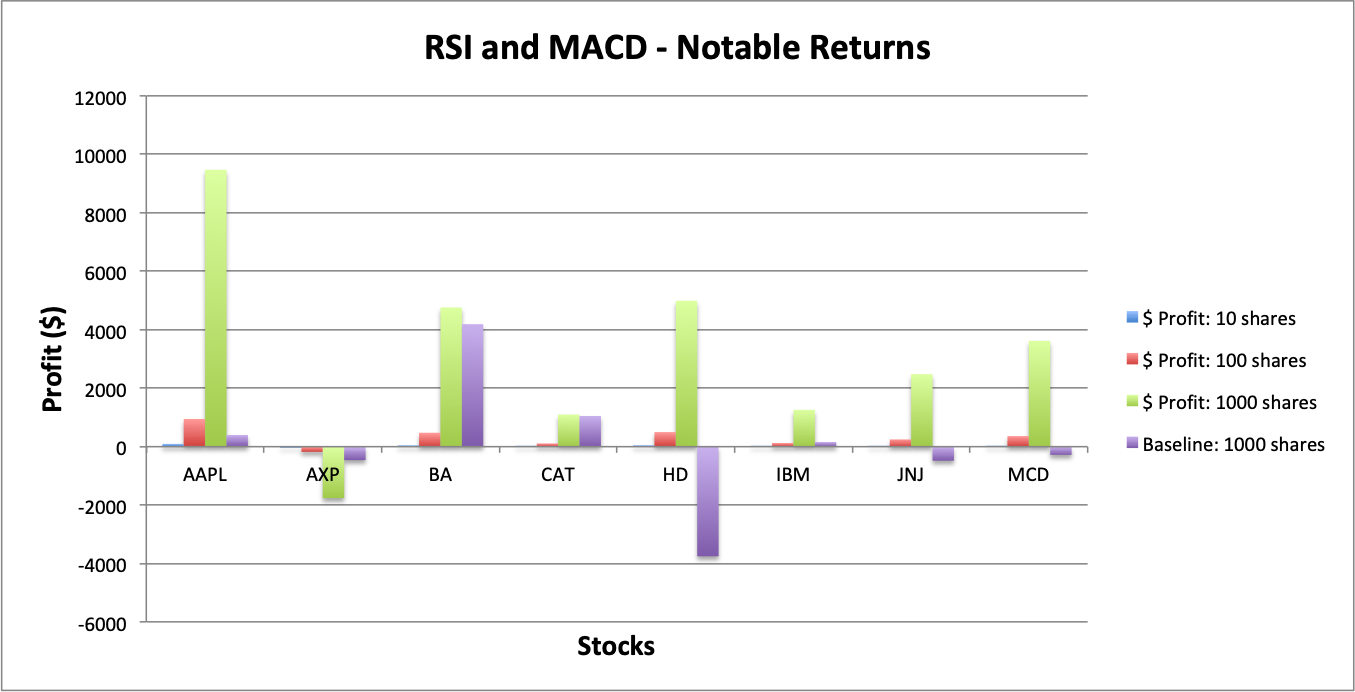
\includegraphics[width=.9\textwidth]{rsimacdresults.png}
\caption{RSI and MACD strategy   \label{overflow}}
\label{RSIMACDRESULTSfigure}
\end{figure} 

\section{Pairs Trading}

Just like the above strategy, our pairs trading implementation performed incredibly well. Compared against the baseline of SPY, a mutual fund that is the industry standard for baseline comparison of AT strategies, this strategy has amazing performance. When using AMD against SBUX, the strategy profited 2143.28\%. QCOM and SBUX performed similarly - culminating in 1748.06\% returns. However, even the lowest performing combination, AMD and VOD, beat out the baseline by over 138\%. Figure~\ref{PAIRSRESULTSfigure} shows these truly astounding results. Furthermore, this strategy would need to be tested on a larger pool of stocks, as only 5 combinations of stocks were cointegrated enough to justify trading together. 

This highlights a common trend. More involved strategies that use multiple measures or inputs always perform better than single measures and nearly always beat the baseline. Just like the combination momentum strategies, the results are incredible. With both pairs trading and as well as the above strategy, someone who implements either strategy could make incredible profits. The barrier to entry however for individuals to truly generate these massive profits, is being able to access up to the minute stock data. All data found via the internet or Quandl is delayed by upwards of 20 minutes, which can make the difference between thousands of dollars and profits and thousands of dollars of losses. However, because pairs trading uses closing prices, one wouldn't have to pay for the end of day closing data.

\begin{figure}[h]
\centering
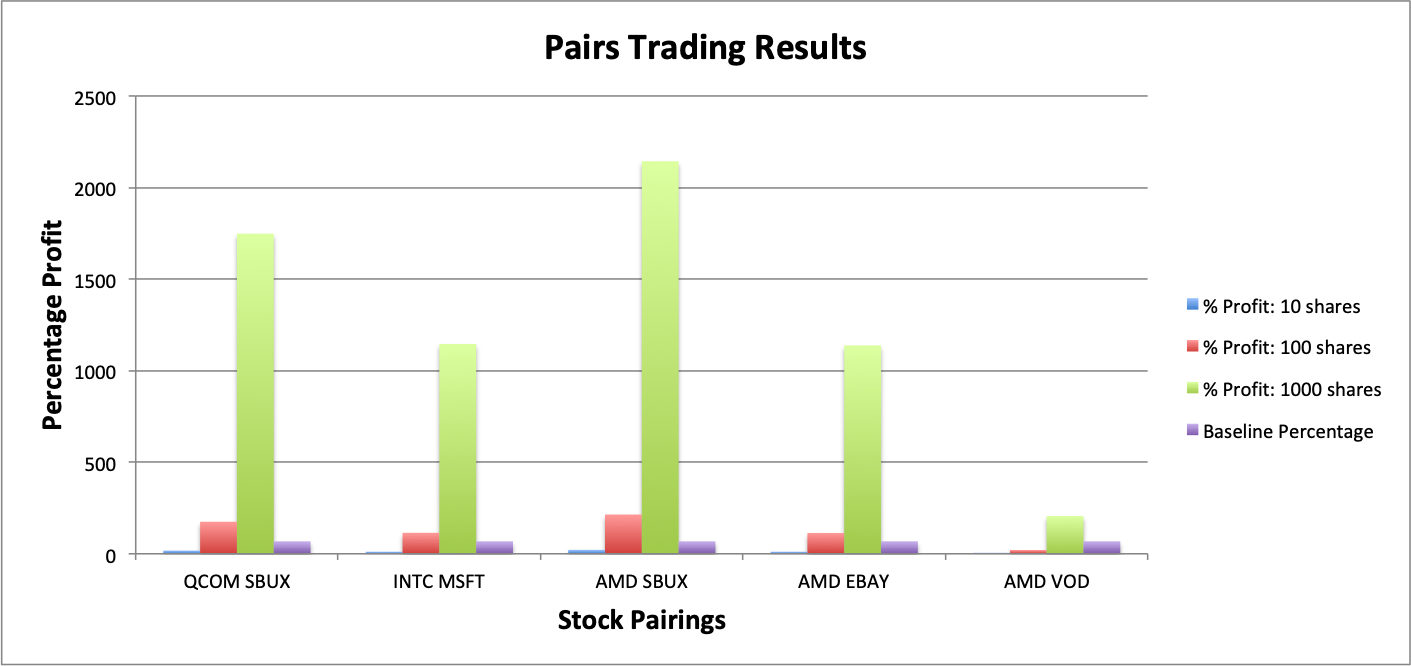
\includegraphics[width=.9\textwidth]{pairstradingresults.png}
\caption{Pairs Trading Results \label{overflow}}
\label{PAIRSRESULTSfigure}
\end{figure}

\end{document}
